\section{DC motoren}
Dette appendix beskæftiger sig med bestemmelsen af motorparametrene.
\subsection{DC Motor karakteristik}
DC Motoren kan modelleres efter diagrammet på fig. \todo[inline]{kredsløbsdiagram skal indsættes}\todo[inline]{Kildehenvisning til DC motor model}.
Ligningen for $V_m$ er givet ved ligning \ref{eq:Vm_transient0}.
\begin{equation}
	V_m(t)=L_m \cdot \frac{\mathrm d}{\mathrm d t} \big( i_m(t) \big)+R_m \cdot i_m(t) + V_{EMF}(t)
	\label{eq:Vm_transient0} 
 \end{equation}
Den modelektromotoriske kraft, $V_{EMF}$ er givet ved ligning \ref{eq:VEMF}.
\begin{equation}
	V_{EMF}(t) = K_b \cdot \omega(t)
	\label{eq:VEMF}
\end{equation}
Med ligning \ref{eq:VEMF} kan ligning \ref{eq:Vm_transient0} omskrives til ligning \ref{eq:Vm_transient1}.
\begin{equation}
	V_m(t)=L_m \cdot \frac{\mathrm d}{\mathrm d t} \big( i_m(t) \big)+R_m \cdot i_m(t) +K_b \cdot \omega(t)
	\label{eq:Vm_transient1} 
 \end{equation}

\subsection{Eksperiment 1}
\subsubsection{Formål}
Bestemmelse af motorens ækvivalente resistans, $R_m$.
\subsubsection{Teori}
Forhindres motoren i at rotere, vil vinkelhastigheden være nul.
Hvis man påfører motoren en DC-spænding $V_m$,
og venter til motorens respons har nået steady-state,
så vil strømmen igennem motoren være konstant.
Her vil ligning \ref{eq:Vm_transient1} kunne omskrives til ligning \ref{eq:resistans_E1}.
\begin{equation}
	V_m=R_m \cdot i_m
	\label{eq:resistans_E1} 
 \end{equation}
Målinger af sammenhørende steady-state værdier for strøm $i_m$ og spænding $V_m$
kan altså bruges til bestemmelse af den ækvivalente resistans $R_m$.
\subsubsection{Fremgangsmåde}
Motoren låses fast vha. en skiftenøgle og påføres en lav spænding.
Efter nogle sekunder, når transientresponsen er væk,
måles spændingen over og strømmen igennem motoren med multimetre.
Værdierne noteres, og forsøget gentages ved andre spændinger.

De anvendte multimetre er af typen TTi 1604.
\subsubsection{Måleresultater}
I tabel \ref{tb:resistans} findes målingerne af strøm og spænding.
\begin{figure}[th!]
	\centering
	%\begin{tabular}{r|r}
%$V_m$ [V]&$i_m$ [A]\\\hline
%0,509&0,094 \\ %0,5093&0,094 \\
%0,883&0,172 \\ %0,8833&0,172
%1,481&0,297 \\ %1,4809&0,297 
%1,940&0,391 \\ %1,9404&0,391
%2,345&0,470 \\ %2,3448&0,470
%2,788&0,555 \\ %2,7879&0,555
%3,182&0,638 \\ %3,1823&0,638
%3,465&0,664 \\ %3,4652&0,664
%3,835&0,746 \\ %3,8346&0,746
%4,067&0,765 \\ % 4,067&0,765
%4,292&0,830 \\ %4,292&0,830 
%\end{tabular}


\begin{tabular}{r|r|r|r|r|r|r|r|r|r|r|r}
$V_m$ [V]&0,509&0,883&1,1481&1,940&2,345&2,788&3,182&3,465&3,835& 4,067&4,292\\\hline
$i_m$ [A]&0,094&0,172&0,297 &0,391&0,470&0,555&0,638&0,664&0,746&0,765&0,830
\end{tabular}
	\captionsetup{type=table}
	\caption[Sammenhørende værdier af DC spænding og strøm]
			{Sammenhørende værdier af DC spænding over og strøm gennem rotationslåst motor.}
	\label{tb:resistans}
\end{figure}
\subsubsection{Databehandling}
Den målte strøm-spændingskarakteristik for DC-motoren er indtegnet på figur \ref{fig:resistans0}.
\begin{figure}[th!]
	\centering
	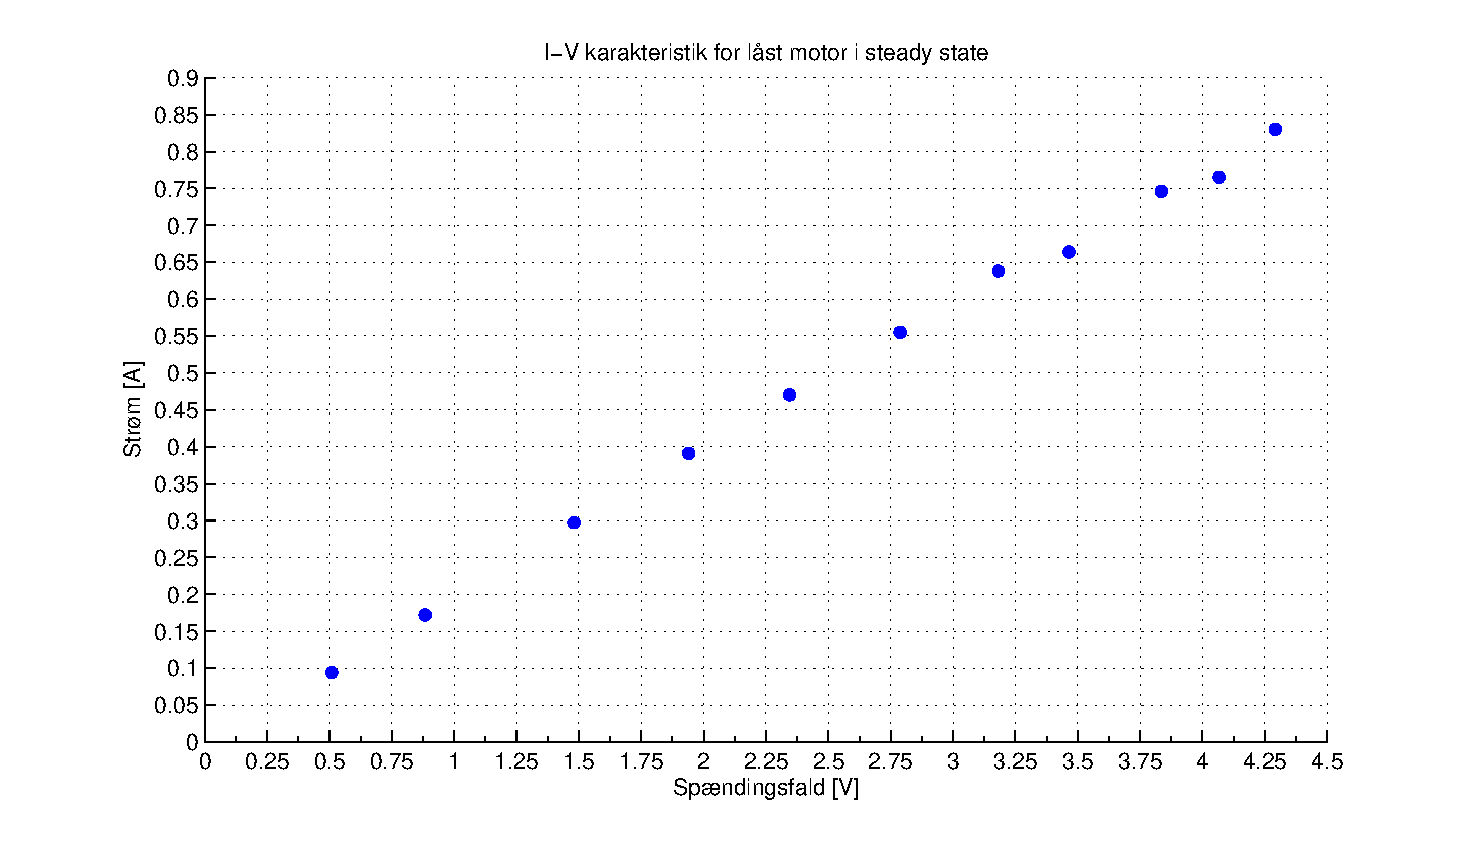
\includegraphics[width=1\textwidth]{./graphics/resistans1.eps}
	\caption[Strøm-spændingskarakteristik for rotationslåst DC-motor]{Strøm-spændingskarakteristik for rotationslåst DC-motor ved steady-state.}
	\label{fig:resistans0}
\end{figure}
Som det ses på figur \ref{fig:resistans0} er sammenhængen mellem strøm og spænding
tilnærmelsesvis lineær, og en lineær regression på dataene vil altså give en tilnærmet værdi for $R_m$.
$R_m$ er ved lineær regression beregnet til 5,21 $\Omega$.\todo{Flere decimaler?}

Den i forsøget mindste afsatte effekt i motoren er 48 mW.
\subsubsection{Diskussion}
Da sammenhængen mellem strøm og spænding i målingerne er tilnærmelsesvis lineær,
vurderes den fundne værdi for $R_m$ at være meget nøjagtig,
om ikke andet, så for effektafsættelser i motoren på mindst 48 mW.
\subsubsection{Konklusion}
Motorens ækvivalente resistans, $R_m$ er vha. sammenhørende målinger af strøm og spænding
for en rotationslåst motor, ved effektafsættelser på 48 mW og højere,
blevet bestemt til 5,21 $\Omega$.\todo{Flere decimaler?}
\subsection{Eksperiment 2}
\subsubsection{Fremgangsmåde og forsøgsopstilling}
\subsubsection{Databehandling}
\subsubsection{Konklusion}


\subsection{Eksperiment 3}
\subsubsection{Fremgangsmåde og forsøgsopstilling}
\subsubsection{Databehandling}
\subsubsection{Konklusion}


\subsection{Eksperiment 4}
\subsubsection{Fremgangsmåde og forsøgsopstilling}
\subsubsection{Databehandling}

\subsubsection{Konklusion}

\subsection{Opsummering af DC motorparameter}